In this chapter we will be exploring the process of designing the experiments and the environments for their execution, as well as presenting the results at the end of it. Firstly, we are addressing the motivations behind choosing the datasets implemented during the set-up. Secondly, the transformations and methods used during the experiments are also discussed with the aim to provide feedback on their use and the possibilities that they offer. Finally, the Results have been placed at the end on this chapter, illustrating the procedures and concepts introduced during this Bachelor's Thesis.

\section{Dataset Selection and Exploratory Analysis}

Before diving into the application of the Autoencoder, we first have to take a look into the data that we will be using on our project. We want to use a wide variety of them to test our tool in order to find out if the assessments made on the previous section hold when applied on some of the most commonly datasets used in the industry. When selecting between the huge amounts of information available online, it was our interest to prioritize them according to a series of qualities. They needed to:
 
\begin{itemize}
	
\item[$\bullet$] Have different instance cardinalities, ranging from easily handable datasets (Iris) to more complex and computational harder (MNIST).

\item[$\bullet$] Different classification task types, from binary to categorical.

\item[$\bullet$] Clearly distinct balance in the datasets, which will help us understand the potential of our tool.

\end{itemize}

The following section will help understand these points and its implications for our task. To do so, a brief description of them and their role on achieving our desired results will be stated. Descriptions of each dataset will include statistics on their distributions as well as why they were chosen as a viable candidate for our goal. Mainly we will be relying on simple computations, such as the median, and trying to plot histograms or similar figures to have visible and more user friendly inputs to understand why some steps will be applied on future scripts.\par
 
This task is necessary if we want to have a hint of the outcome of the processes that will take place on the datasets, as well as to shed  light onto the difficulty to adapt our scripts and architectures when moving from one dataset to another one. It also provides some information about why they were chosen as viable candidates in our experiments.

 

\subsection{Anderson's Iris}

(Anderson's) Iris is a multivariate dataset published in~\cite{Fisher_Iris}. The data itself consists of 50 samples from each of three species of Iris: \emph{Iris setosa}, \emph{I. virginica} and \emph{I. versicolor}. Each exemplar had four of their characteristics recorded: the length and the width of the sepals and petals in centimetres. \par

Based on the distribution of the measurements obtained from the dataset, Fisher's data has been referred to as one of the basic staples of data classification due to the fact that it is divided into two clearly differentiable clusters, one containing Iris setosa and the other one including both virginica and versicolor. Without the labels provided by Fisher, the classifying task becomes more complex. This feature is specially useful to highlight the differences between unsupervised and supervised classification tasks. %\newline
% 
\begin{table}[H]
		\caption{R's summary method on Iris.}
	\begin{center}
	\label{tab:table_Iris}
		\begin{tabular}{r|c|c|c|c} % <-- Alignments: 1st column left, 2nd middle and 3rd right, with vertical lines in between
			\textbf{Variable name} & \textbf{Sepal Length} & \textbf{Sepal Width} & \textbf{Petal Length} & \textbf{Petal Width}\\
			\hline
			Minimun & 4.30 & 2.00 & 1.00 & 0.10\\
			Median & 5.80 & 3.00 & 4.350 & 1.30\\
			Mean & 5.84 & 3.06 & 3.76 & 1.20\\
			Maximun & 7.90 & 4.40 & 6.90 & 2.50\\
		\end{tabular}
	\end{center}
\end{table}

Table~\ref{tab:table_Iris} contains summaries of the features of iris, and by looking at them we can already see that the data is very balanced on every feature as the distance between the minimum and the maximum divided by two is approximately the Mean, which also has a close value to the Median. To us, this means that the data is centred over a certain value, which will allow us to simplify our tasks by doing some type of translation transformation over the data before fitting it through our tools. Regardless, plotting will also help us discern the real difficulty of our classification task.
%
\begin{figure}[H]
	\centering
	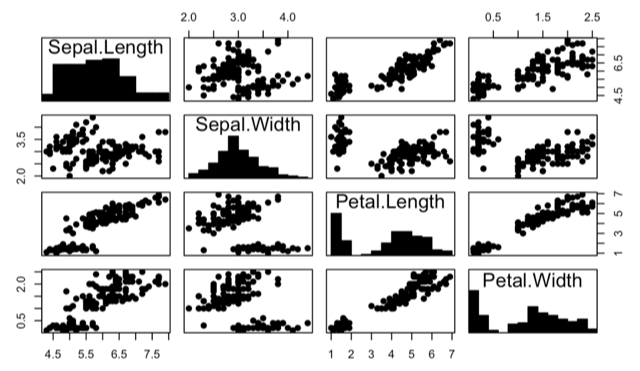
\includegraphics[width=13cm]{Figuras_tfg/Figure_Iris_Histogram}
	\caption{Using the pairs function summary}
	\label{fig:figure_pairs_iris}
\end{figure}


Taking a look at Figure~\ref{fig:figure_pairs_iris}, The histogram in the middle is showing some higher values in different ranges on our data. If we hadn't observed the summary values in Table \ref{tab:table_Iris} , we could have struggled with coming up with a general idea behind the dataset. But sometimes histograms are a little bit more troubling to read into, so plotting Figure~\ref{fig:figure_knn_classifier} can help understand the relationships between classes and their features. For example, the iris dataset would be a good fit for a knn classifier, as its data classes and observations are clearly distinguishable when using Petal Width and Petal Length rather than when using Sepal Width and Sepal Length. 
%
\begin{figure}[H]
\begin{minipage}{.5\textwidth}
        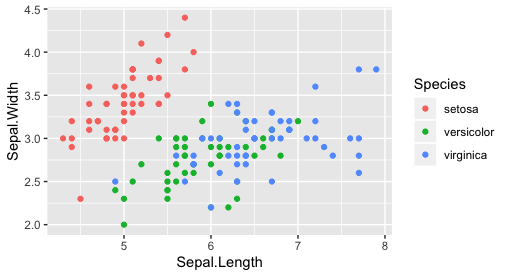
\includegraphics[scale=.54]{Figuras_tfg/R_plot_iris_knn_width_sepal}
 \end{minipage}%
 \begin{minipage}{.5\textwidth}
        \begin{flushright}
               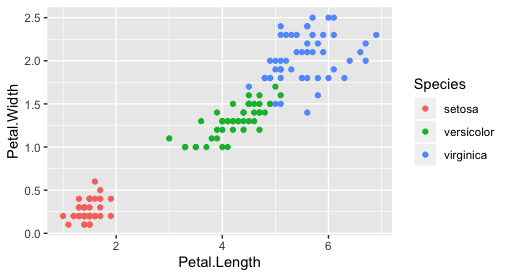
\includegraphics[scale=.54]{Figuras_tfg/R_plot_knn_petal}  
        \end{flushright} 
    \end{minipage}  
  \caption{Plotting of two different features of Iris with respect to the class label. As it can be seen here, depending of how you organise your data you can get more efficient classifiers and clusters. }
 \label{fig:figure_knn_classifier}
\end{figure} 

\subsection{MNIST}
\label{subsec:MNIST}


The MNIST dataset~\cite{MNIST_article} is a large database of handwritten digits widely used in Data Science for experimenting. It is mostly used for image processing and it is composed by samples of handwriting taken from the National Institute of Standards and Technology original datasets. It was later normalized to fit into 28x28 pixel images. Every image has vector $X$ of values $24 \times 24 = 784$ between 0 and 255 ,which defines the shape and shades of grey of the number in the image. Then, the $Y$ class contains vectors with a character which can be related to its corresponding pixelized image by a classification method. \par

The database contains 60\,000 training images and 10\,000 testing images for $X$ and $Y$. Many different authors~\cite{MNIST_classification_example}, have tried to achieve the lowest error rate on it. Convolutional neural networks managed to get a very low error of around $0.23$, although other methods such as support-vector machine get an error of as low as $0.56$ too~\footcite{wiki:MNIST}.
%
\begin{figure}[H]
\centering
  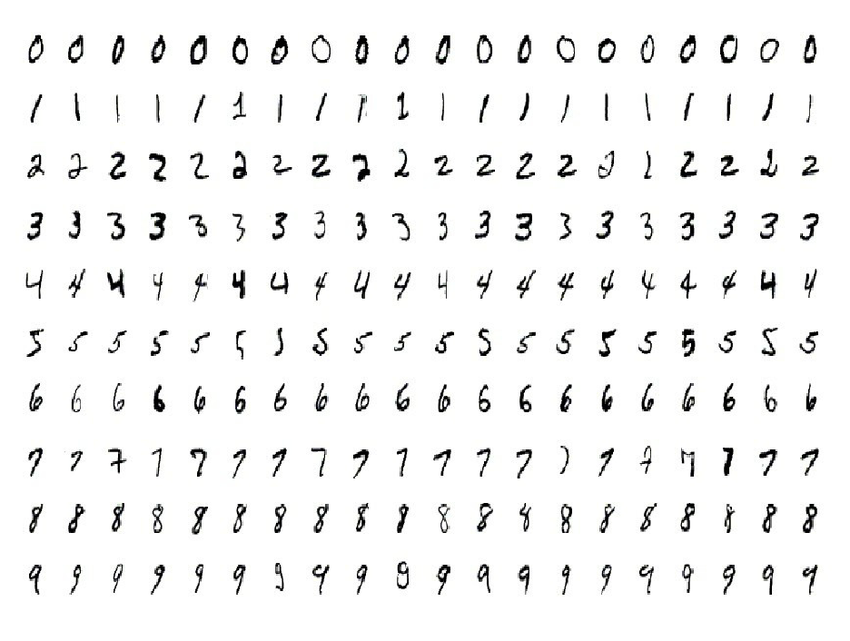
\includegraphics[width=16cm]{Figuras_tfg/Figure_MNIST}
  \caption{Some examples of the images included in the MNIST dataset}
 \label{fig:figure_MNIST}
\end{figure}

Using the previously mentioned summary method on the training vectors for $X$ on this particular dataset will not provide us with enough information to estimate the classification task complexity. As we can see from Table~\ref{tab:table_MNIST}, we just know the range of values of every image (already studied in the definition of the dataset) and the mean, which only states that out training pixels tend to be white rather than black, the reason being that the characters are written over white paper. In this case, since all of our bits are grey values)
, it is on our best interest to try to simply our task by dividing our training and test numbers into binary representations of their types. Achieving it will only mean to transform them into 1s and 0s, and easier representation to handle for our transformation block. 
%
\begin{table}[H]
	\caption{R summary method on MNIST.}
	\begin{center}
		\label{tab:table_MNIST}
		\begin{tabular}{r|c|c|c|c} % <-- Alignments: 1st column left, 2nd middle and 3rd right, with vertical lines in between
			\textbf{Variable name} & \textbf{Minimun} & \textbf{Median} & \textbf{Mean} & \textbf{Maximun}\\
			\hline
			X training & 0 & 0 & 33.32 & 255 \\
			X testing  & 0 & 0 & 33.32 & 255 \\
		    Y training & 0 & 4 & 4.454 & 9 \\
		    Y testingg & 0 & 4 & 4.443 & 9 \\
		\end{tabular}
	\end{center}
\end{table}


If we instead observe the summary from the $Y$ training data we can see that the dataset is very balanced, as the mean is close to half of the distance between the Minimum and the Maximum. This tells us that we will be able to probably achieve high degrees of accuracy on our classifier, as well as that the Entropy Triangle should also perform a satisfying job when analysing its informational flows.  \par

Our goal when fitting MNIST  through the autoencoder is to asses its capabilities when using bigger chunks of data and compressing it. Numerous reports and information available online give plethora of information about possible classification methods and their expected outcome in terms of error rates and accuracy. 
%
%We are not trying to improve their results, we are just mimicking their processes and applying some of their methods so that we can achieve similar results when applying our tools.\par

\subsection{Ionosphere}
\label{subsec:Ionosphere}

Ionosphere represents a set of data collected by a radar in Goose Bay, and later used for data science purposes by the Johns Hopkins University~\cite{Sigillito1989ClassificationOR}. The antenna had a phase array of 16 high-frequency antennas and used times pulses and pulse numbers for processing. The outputs can be labeled as either "good" or "bad", referring to the fact that a radar signal going through the ionosphere and thus showing no evidence of the existence of an ionosphere was labeled as "bad", and in any other case we would be labeling it as "good". It can be found on the R package "mlbench". %\newline
%
\begin{figure}[H]
	\centering
	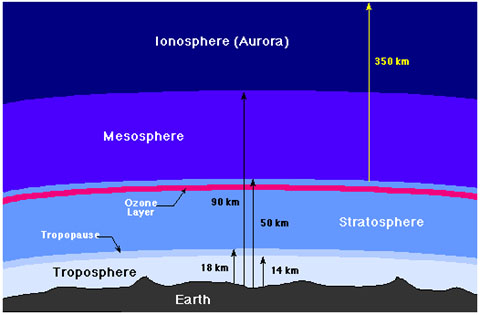
\includegraphics[width=10cm]{Figuras_tfg/Ionosphere}
	\caption{The Ionosphere is one of the main layers composing Earth's atmosphere}
	\label{fig:figure_pairs_ionosp}
\end{figure}

There are 351 observations from 35 independent variables, with 33 of them being numerical values and 2 of them representing nominal values (one of them defining the class). However, one of the variables included in the dataset can be safely removed since it only represents a constant value (0). Having removed that one it should be remarked that this dataset is not balanced, since we don't posses the same number of ``good'' or ``bad'' class labels, and the difference is big enough to potentially affect its transformation and classification. We can expect its performance to be worst than the other two datasets mentioned previously. In the Ionosphere case, we will classify our data using binary decision, as there are only two states available for our labels. \par

Researchers have found very high accuracies when using non-linear perceptrons on this dataset~\cite{Sigillito1989ClassificationOR}, by using the same quantities of "good" and "bad" observations, which would not fit our needs. Although it can be easily inferred that we are going to get some degenerated results when compared with other papers, it seems like an appropriate choice to check the performance of the Entropy Triangle. \par 

\section{The classifiers}
\subsection{K-Nearest Neighbours}

K-Nearest Neighbours (KNN) is a non-parametric supervised classification method used for estimating the density function~\cite{mur:12}. As an supervised algorithm, it needs labelled data to learn the appropriate function that produces new data belonging to the different regions of the existing classes when introducing new unlabelled data. Depending on the desired predictors we will want to obtain either a regression or a discrete output in our classifier. 

The KNN algorithm hinges on the assumption that similar data must be close in a metric space representation. This hypothesis means that, in practice, we must take into account that proximity will be primordial to the outcome of our classification process when we are using the KNN classifier. This particular way of solving a data analysis problem is specially interesting when the data we are trying to analyse is very close to the same labelled data, since KNN relies in a ``majority voting'' scheme to predict the class for a sample using $K$ nearest neighbour samples---hence the name of the technique---, where $K$ is a fixed parameter of each run of the algorithm. 

Although the majority voting classification method has some positive advantages~\cite{article_voting_algorithms}, it also comes with some drawbacks too: in those cases where the class distributions are skewed, we can end up with a class which solely dominates the predictions. There are many ways of overcoming this issue, such as assigning proportional weights or to build clusters with similar points, but the reality is that KNN has a defined scalability that depends on the noise of your data and the characteristic of your dataset~\cite{Knn_characteristics}. \par

In order to try to improve results and polish the overall performance of the algorithm there are some tricks to take into account and follow when designing it: 

\begin{itemize}
	
	\item[$\bullet$] Trying to fit data through multiple instances of your implemented algorithm with new values for $K$ in each case.
	
	\item[$\bullet$] Avoid using even $K$'s values when doing binary classification, as we want to avoid tied votes.
	
	\item[$\bullet$] Perform an exploratory analysis of your data and design the boundaries and expected performance of your algorithm. Sometimes, realizing that a problem will be very lengthy and tedious to solve using a pre-determined method will save you a lot of time .
	
\end{itemize}

\begin{figure}[H]
	\centering
	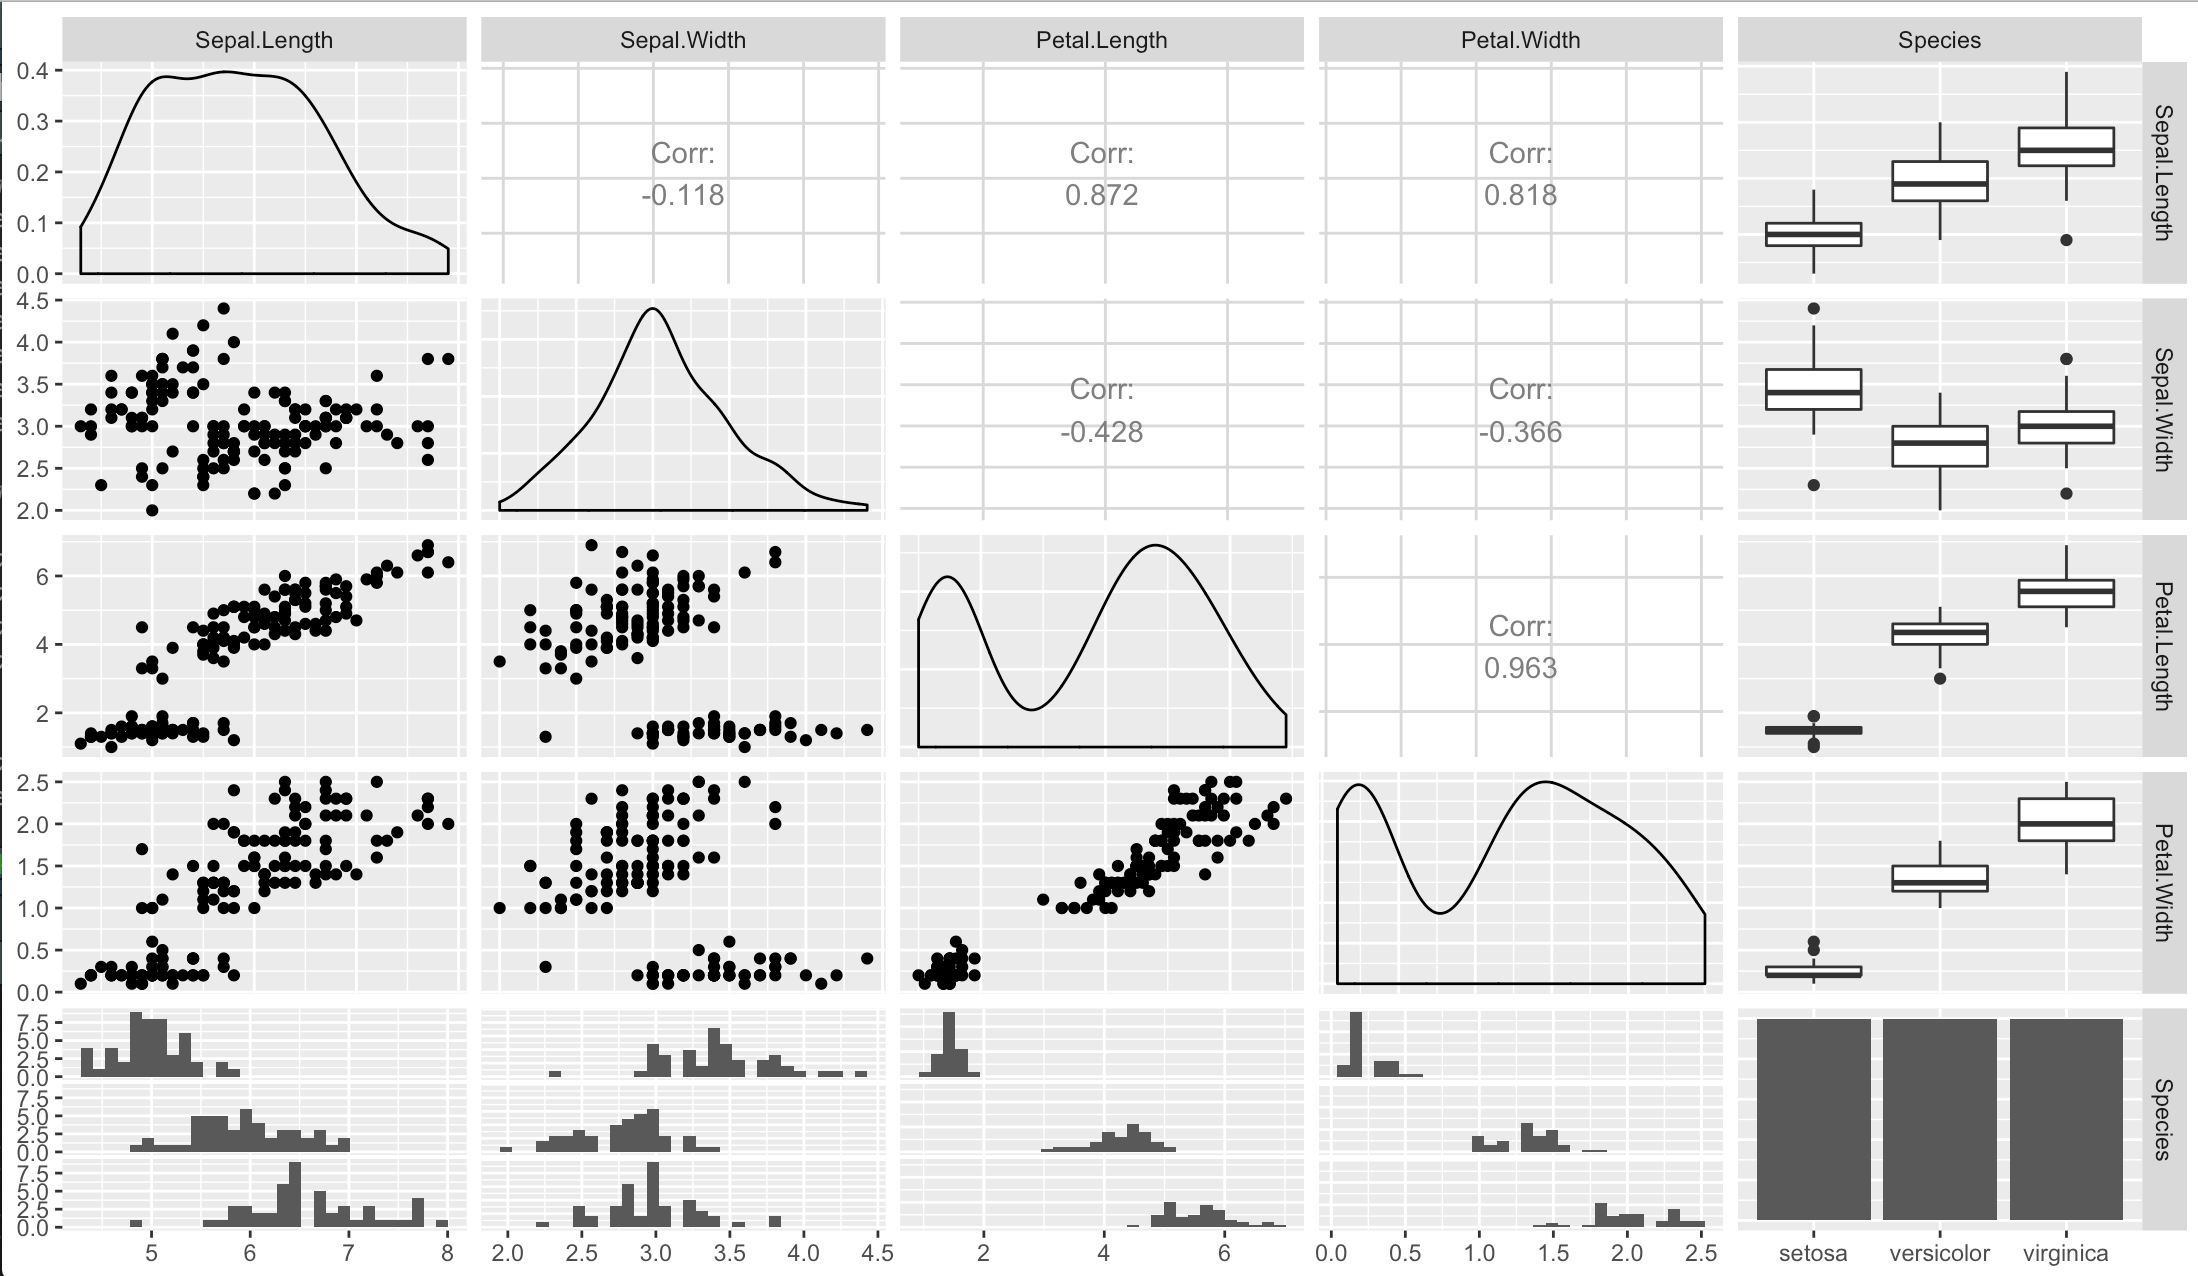
\includegraphics[width=15cm]{Figuras_tfg/R_plot_correlation.png}
	\caption{The GGally R package also provides useful tools for this types of problems. Here, the correlation between \textrm{Petal.length} and \textrm{Petal.Width} is proven to be very high, as the plots from Figure~\ref{fig:figure_knn_classifier} showed}
	\label{fig:figure_knn_classifier_correlation}
\end{figure}

\subsection{Multilayer Perceptron}

The Multilayer Perceptron (MLP) has a similar architecture to that of DNNs. Both of them have input, output and hidden layers as well as having nodes and using back-propagation for training. They even need their layers to be activated, as well as support the most common functions used in the Autoencoders. It can even be considered it as a slightly less computationally powerful DNNs. \par

It would seem as the main interest into MLPs could be to use them for smaller Autoencoders, but actually they possess a very important feature: they  can distinguish and classify data that is not linearly separable.This property can help us qualify and compare different types of classification tasks~\cite{MLP_classifier}. As it is interesting to test multiple algorithms to make the most out of our ET, we can may compare them  to the rest of the classifiers presented in this Section. It can be especially useful when we compare it with a  KNN classifier, and we will implement both of them in our project to perform the same classification tasks over the same datasets. We would expect it to generally perform better on more complex datasets than KNN, which suffers when data is more difficult to differentiate. \par

\section{Principal Component Analysis}

\subsection{Description}
Principal Component Analysis (PCA) is a statistical procedure based on orthogonal transformations to convert observations of possibly uncorrelated variables into sets of linearly uncorrelated variables called \emph{principal components}. The transformation is performed in such a way that the first component has the largest possible variance, with each succeeding component having the highest variance taking into account that it has to be orthogonal to the preceding components. We will finally end up with a set of vectors which are uncorrelated. Due to the nature of the transformation, PCA can be affected by any type of scaling of the original dataset~\cite{mur:12}. 
%
We also know that this method is valid to asses the capabilities of the ET due to the fact that it's use has already been introduced into experiments~\cite{val:pel:18c}.

PCA is used in the data analysis field for Exploratory (EDA) or Confirmatory Data Analysis (CDA)\footnote{Modernly called ``Predictive Data Analysis''.}~\cite{tuk:80}. It can be used to visualize the genetic distance between populations of data. Results from the PCA are usually discussed taking into account their components. Other characteristics include:

\begin{description}
	
	\item[$\bullet$] PCA is a simple eigenvector-based multivariate analysis. This is specially important to our task since this operation can help us discern the real structure of the data. It can also reduce the dimensionality of the data to view its most informative components and features.
	
	\item[$\bullet$] It resembles factor analysis~\cite{PCA_and_factor_analysis}. Both of them are used to describe the variability of the data and reduce its dimensionality, but use different techniques to reach that goal.
	
	\item[$\bullet$] It also resembles canonical correlation analysis (CCA)~\cite{PCA_and_CCA}. While CCA tries to describe the cross-variance between two datasets, PCA defines the variance of a single dataset by using an orthogonal coordinate system.
	
\end{description}

\subsection{PCA and Information Theory}

Our goal when using PCA in this project is to compare the results of the Autoencoder with another widely used tool in the data science field. At the same time, we want the theoretical underpinnings to be tacit on both methods used so that the outcome can be correctly compared when using the Entropy Triangle.\par

PCA fulfils our requirements by trying to minimize  informational losses. If we assume our model vectors to be defined by the  following equation :
%
\begin{equation}\label{eq:pca_equation}
\vec x = \vec s + \vec n 
\end{equation}
\noindent
where $\vec x$ represents the vector being the sum of the desired information-bearing signal $\vec s$ and a noise (multivariate) signal $\vec n$. If we use this equation, it can be assumed that our vector can be dimensionally reduced.\par

For this model to hold true, the noise $\vec n$ has to be multivariate Gaussian with a covariance matrix proportional to the identity matrix. This fact allows us to maximize the mutual information between the dimensionally reduced output $\vec y$ and our $\vec s$ signal, only if we consider that the same assumptions made for $\vec n$ also apply for $\vec s$. \par

On the other common scenarios, on which $\vec s$ is not Gaussian, at least we will have an upper-bound for our representation such as,
%
\begin{equation}
\label{eq:pca_upper_bound}
I(\overline X; \overline S) - I(\overline Y; \overline s)
\end{equation}
\noindent
Recall that mutual information is defined on random vectors, in general, e.g. for $\vec x$ being a realisation of $\overline X$.


If our noise is dependent, the PCA looses its informational properties and thus we cannot use the previous representation. On the other hand, if our noise is more akin to a Gaussian than our information-bearing signal $\overline S$, our PCA representation will be improved.

